\section{Narrow focus (Theorem~\ref{thm:narrow})}
\label{sec:narrow}

\subsection{Technical form and the rule}

\begin{proposition}[narrow focus, line form] \caproofst{Sec.~\ref{sec:ca} and App.~\ref{app:C}}
\label{prop:narrow}
Let $\ell\ge55.26$.
Let a state satisfy $\mu>0$, $\sigma^3\le r\le\tfrac14$, $B\ge\max(2.5\times10^{10},\,50(8\ell+100))$, $b\le\tfrac12$, $\kappa>0$, and let $P>0$ satisfy (H$'$) (Lemma~\ref{lem:Hprime}).
Then for every $a\in(0,4r/\sigma]$ the option $k$ chosen by the rule below satisfies $\Lambda_k(a)\ge0$ with $\gamma=\Gamma_\ell$.
There is no upper limit on $\ell$.
\end{proposition}

\emph{The rule.}
Put $c_1=0.78$, $c_T=3.5$, $c_{\rm ch}=2.9$, $\Gamma_2=\Gamma_\ell k_2$, $a_s=4c_m^2\ell^6\sigma^3/r$ with $c_m=2X_1\sqrt{2+r}/((1-\eta)\,\mathrm{fl}\,(1-z_2/2)\sqrt{2\pi})$.
\begin{itemize}
\item \emph{Case I} ($G\le c_1\sqrt b/\Gamma_2$): if $b<0.1$ and $\kappa\ge c_T\sqrt\ell\,b/\sigma$, use Tz-B2; otherwise Fz.
\item \emph{Case II} ($G>c_1\sqrt b/\Gamma_2$): if $r\le c_{\rm ch}\sqrt\ell\,\sigma$, use Tz-B2 for every $a$; otherwise Tz-B2 for $a<a_s$ and Tz-B1 for $a\ge a_s$.
\end{itemize}
In Case~I the ripple is dark against the background, and the two background lines P1 and P4z pay for the target.
In Case~II the ripple is brighter than the background; the ripple lines P2z, hFz and the chirp cKz are needed.

\begin{proof}[Proof of Theorem~\ref{thm:narrow} from Proposition~\ref{prop:narrow}]
If $G>0$, Lemma~\ref{lem:lines} and Proposition~\ref{prop:narrow} give $(\mathrm{Num}-\Gamma_\ell\sigma\,\mathrm{den})/\sigma\ge\Lambda_k(a)\ge0$ at the state's own $a=4\sigma/L^2$.
If $G=0$, Lemma~\ref{lem:G0} gives $(a)+(a')\ge0.1995>\Gamma_\ell$.
\end{proof}

All numbers below are values at $\ell=55.26$, which is the hardest point for almost all of them.
That every quoted number and every condition holds for \emph{all} $\ell\ge55.26$ is the computer-assisted part (Sec.~\ref{sec:ca}).
Quantities that contain $B$ are bounded uniformly with $B\ge2.5\times10^{10}$, $q\le(1+\eta)/(400(1-\eta))$ and $z_2\le0.01$.

\subsection{Ceilings from the brightness hypothesis}

\begin{itemize}
\item[(F1)] $P\le0.7008$. In (CM), $\hat E\le1/16$, $E\ln(2B_0/E)$ increases on $(0,1/16]$, $B_0$ increases in $b$, and $B_0(1/16,1/2)=2.25$; hence $P\le2[(1.25/16)\ln72+c_{\rm CM}/2]$.
\item[(F2)] If $\max(\kappa,16b)\le\kappa_b\le1$, then $P\le w_{16}\sqrt{\kappa_b}$ with $w_{16}=e^{1/2}[(1+1/32)(1/8)\ln(32B_0(1/16,1/16))+2c_{\rm CM}/16]\le0.8972$ ((J) with $\lambda=1$).
\item[(F3), (F4)] Lemma~\ref{lem:DI}, items (iv)--(v) and (K).
\end{itemize}

\subsection{Remainders}
\label{sec:R}

With $\mathrm{es}=10^{-11}$ and $\mathrm{es}_\sigma=\ell^2e^{-\ell}$:
\begin{itemize}
\item[(R1)] N1 $=\varepsilon_1(r)\,$P1 with $\varepsilon_1\le0.01457$; the other L-lines satisfy $\mathrm{N2}+\mathrm{d3}+\mathrm{N4}+\mathrm{ring2}+\mathrm{A2a}+\mathrm{A2b}+\mathrm{B2b}\le0.52\,\mathrm{es}\,$P1, the largest part being $\mathrm{N2}/\mathrm{P1}=Q_2/(8B)\le0.507284\,\mathrm{es}$; d4$+$N4G and B1l are at most $\mathrm{es}_\sigma\,$P2z.
\item[(R2)] hneg1 $=\varepsilon_h(r)\,$P4z with $\varepsilon_h\le0.1808$.
\item[(R3)] The S-lines are $c_Sb\sqrt{\sigma a}$ with $c_S\le0.155$, at most $0.48\,\mathrm{es}$ times P4z ($a\le1$) or P1 ($a\ge1$).
\item[(R4)] The constant lines satisfy $\mathrm{N3}+\mathrm{M0Xi}+\mathrm{A1v}+\mathrm{pair}\le1.77\sigma$. With $e_0=1.26\times10^{-5}$, $m_1=1-\varepsilon_1-e_0$, $m_4=1-\varepsilon_h-e_0$, for all $a\ge0$
\begin{equation}
\begin{split}
&(1-\varepsilon_1-\mathrm{es})\frac a2+(1-\varepsilon_h-\mathrm{es})\frac{b\omega/2}{a+\sigma}-1.77\sigma\\&\qquad\ge\ m_1\frac a2+m_4\frac{b\omega/2}{a+\sigma},
\end{split}
\end{equation}
because $\mathrm{P1}+\mathrm{P4z}\ge\sqrt{b\omega}-\sigma/2\ge1.58\times10^5\sigma$ when $B\ge2.5\times10^{10}$. This is where the lower end of $B$ is used.
Then $m_1a/2+m_4(b\omega/2)/(a+\sigma)\ge\sqrt{m_1m_4b\omega}-\sigma/2\ge\Gamma_\ell bk_1+c_{1F}\sqrt b$ with $c_{1F}\ge0.7857$.
\item[(R5)] In Case~I, if $b\ge0.1$ or $\kappa<c_T\sqrt\ell\,b/\sigma$, the loss of Fz is $K_F=\mathrm{FzK}+\mathrm{A2k}+\mathrm{B2a}\le1.01\times10^{-3}\sqrt b$ (from $G\le c_1\sqrt b/\Gamma_2$ for small $b$, and from (K) otherwise).
\item[(R6)] For $a\le4r/\sigma$ the branch B2 costs $\mathrm{B2c}+\mathrm{B2s}\le c_{B2}G$, $c_{B2}=X_1/(4\sqrt2(1-\eta))+c_s/(4(1-\eta))\le0.0896\sqrt\ell$. This is where the upper end of $a$ is used.
\item[(R7)] In Case~II with $r>c_{\rm ch}\sqrt\ell\sigma$ and $a\ge a_s$: $\mathrm{B1m}\le\ell^{-3}\,\mathrm{hFz}+\mathrm{es}_\sigma\mathrm{P2z}$, $\mathrm{B1c}\le\mathrm{es}_\sigma\Gamma_2G$, and $\mathrm{uB2c}+\mathrm{uB2s}+\mathrm{A2k}+\mathrm{B2a}\le(c_u\sqrt r+2.1b^2)\,\mathrm{cKz}$ with $c_u\le0.48$.
\end{itemize}
The es-budget is shared: P1 carries $0.52\,\mathrm{es}$ from (R1) and, for $a\ge1$, $0.48\,\mathrm{es}$ from (R3); P4z carries $0.48\,\mathrm{es}$ for $a\le1$.
The lower end $r\ge\sigma^3$ is used only in (R1), through the factors $1/\sqrt r$ of A2b, B2b and ring2.

\subsection{Case I}

\emph{Option Fz.} By (R1)--(R5),
\begin{equation}
\Lambda_{\rm Fz}\ \ge\ (c_{1F}-1.01\times10^{-3})\sqrt b-\Gamma_2G\ \ge\ 0,
\end{equation}
since $G\le c_1\sqrt b/\Gamma_2$ and $c_{1F}-1.01\times10^{-3}\ge c_1=0.78$.

\emph{Option Tz-B2} ($b<0.1$, $\kappa\ge c_T\sqrt\ell b/\sigma$). The background part is the same; it remains to show $\mathrm{cKz}-\mathrm{B2c}-\mathrm{B2s}-\mathrm{A2k}-\mathrm{B2a}\ge0$.
For $b<0.1$, $k_f\ge0.4493$ and $\mathrm{cKz}\ge c_K\kappa\sigma G/b$ with $c_K=\mathrm{fl}\,k_f/16\ge0.02758$; moreover $\mathrm{A2k}\le0.04616\,\mathrm{cKz}$ and $\mathrm{B2a}\le10^{-6}\,\mathrm{cKz}$.
What is needed is $(1-0.04616-10^{-6})c_Kc_T\sqrt\ell\ge c_{B2}$: at $\ell=55.26$ the two sides are $0.6845$ and $0.6656$.

\subsection{Case II forces a chirp}

In Case~II, $G^2>c_1^2b/\Gamma_2^2\ge1.9863\,\ell b$, while $G^2\le(r/2)P^2$.
\begin{itemize}
\item[(c1)] $G\le P/3$ gives $b<c_bP^2$ with $c_b=(\Gamma_2/(3c_1))^2\le0.05593/\ell$; with (F1), $b\le0.0275/\ell$, and (CM) used again gives $P\le P_{\rm II}=0.5223$. Then $\mathrm{brk}\ge0.998$, so the Tz options are available.
\item[(b.1)] For $\mu>5.61$, Lemma~\ref{lem:DI}(v) with $t=\mu/(2A)$ gives $P\le9\mu e^{-0.4\mu}$; two passes of Lemma~\ref{lem:DI}(iv) give, for $\mu\ge7.44$, $P\le4\mu e^{-\mu}E_{\rm CM}$, $E_{\rm CM}=(1+3.445e^{-\mu/2})^2(1+2\times10^{-3}/\ell)$.
\item[(b.2)] $\mu<\ell+\ln\ell$: otherwise $G\le1.5\sigma$, while Case~II has $G\ge2.2\times10^5\sqrt\ell\,\sigma$.
\item[(c2)] If $\kappa\le1$: $\kappa>c_\kappa\ell b/r$ with $c_\kappa=2c_1^2/(\Gamma_2^2\ell w_{16}^2)\ge4.935$ (from (F2) with $\kappa_b=\max(\kappa,16b)$, and $\kappa_b=16b$ is impossible). Hence $\chi>\mathrm{fl}\,k_fc_\kappa\ell\sigma/(16r)$.
\item[(c3)] If $\kappa>1$: $b<(\Gamma_2^2/c_1^2)(r/2)P_{\rm II}^2$, hence $\chi>\mathrm{fl}\,k_fc_1^2\sigma/(8\Gamma_2^2P_{\rm II}^2r)$.
\end{itemize}
In words: a ripple that is brighter than the background cannot keep its brightness at the centre of the focus, because a concentrated ripple is dark (F2).
So in Case~II, $\kappa$ is large compared with $b/r$, and the chirp gain $\chi G$ is always there.

\subsection{Case II, three regions}

\emph{(II-ch) $r\le c_{\rm ch}\sqrt\ell\sigma$, option Tz-B2.}
$\Lambda\ge(1-\mathrm{es}_\sigma)\mathrm{P2z}+\mathrm{hFz}+(1-10^{-3})\chi G-c_{B2}G-\Gamma_2G$, and (c2)--(c3) give $(1-10^{-3})\chi\ge0.1041\sqrt\ell$, while $c_{B2}+\Gamma_2\le0.0996\sqrt\ell$.

\emph{(II-s) $r>c_{\rm ch}\sqrt\ell\sigma$, $a<a_s$, option Tz-B2.}
Here $a_s\le\ell^7\sigma^2\le10^{-9}\sigma$, so $\mathrm{hFz}\ge0.1085(r/\sigma)G\ge0.3149\sqrt\ell\,G\ge(c_{B2}+\Gamma_2)G$.

\emph{(II-m) $r>c_{\rm ch}\sqrt\ell\sigma$, $a\ge a_s$, option Tz-B1.}
Collecting (R), for every $a\ge a_s$,
\begin{equation}
\Lambda_{\rm Tz\text{-}B1}(a)\ \ge\ Xa+\frac{Y}{a+\sigma}+m_5\chi G-\Gamma_2G\,(m_T+T),
\label{eq:IIm}
\end{equation}
with $X=m_1/2+m_2\alpha G$, $Y=m_4b\omega/2+m_3\beta G$, $m_2=1-3\mathrm{es}_\sigma$, $m_3=1-\ell^{-3}$, $m_5=1-c_u\sqrt r-2.1b^2$, $m_T=1+\mathrm{es}_\sigma$ and $T=bk_1/(Gk_2)<0.1877/\ell$.
Write $u=m_1/(2m_2\alpha G)$, $v=m_4b\omega/(2m_3\beta G)$, $\Theta^*=2\sqrt{m_2m_3\alpha\beta}/\Gamma_2$, $\mathrm{ch}=m_5\chi/\Gamma_2$, and $\xi=(r\sqrt\mu/\sigma)\,c_0$ with $c_0\ge0.9974$.
Then $\Theta^*\ge\vartheta_0\sqrt{\ell/(4\mu)}$, $\vartheta_0\ge0.7858$: the two ripple lines alone pay when $\mu$ is small.
The region splits by $\xi$:
\begin{itemize}
\item[(m1)] $\xi<8$: $Y/(2\sigma)\ge0.157\sqrt\ell\,G$ and $\sqrt{2XY}\ge5.5\,\Gamma_2G$, both above $\Gamma_2G(m_T+T)$.
\item[(m2)] $\xi\ge8$ and $\Theta'=\Theta^*(1-\bar\varrho/2)\ge m_T+T$: the arithmetic--geometric mean of the two ripple lines suffices.
\item[(m3)] $8\le\xi<\ell^2$ and $\Theta'<m_T+T$ (narrow states): then $\mu>0.1347\,\ell$, (b.1) applies, and (F4) gives $\chi\ge\mathrm{fl}\,k_fc_J\ell\sigma e^{2\mu}/(16\mu^3E_J^2r)$, $c_J\ge0.0913$. The chirp alone pays: $\mathrm{ch}\ge17$ at $\ell=55.26$, $\mu=7.44$, and $\mathrm{ch}$ increases from there.
\item[(m4)] $\xi\ge\ell^2$ and $\Theta'<m_T+T$ (wide states): then $\mu>0.1531\,\ell$ and $\mu<\ell+\ln\ell$. If $u$ or $v$ exceeds $U=((m_T+\bar T)/\Theta')^2-1\le5.96$ the bound follows. Otherwise $r<18.7E_{\rm CM}^2e^{-2\mu}$ and one of two closings applies.
For $B<\ell^4$ (which occurs only for $\ell>397.6$), (F4) forces $u>6\ge U$ in both sub-cases of $\kappa_b$ ($u\ge6.09\times10^{28}$ if $\kappa_b=\kappa$, $\ln u\ge220$ if $\kappa_b=16be^\mu/\mu$), a contradiction.
For $B\ge\ell^4$, put $\delta=\ell/4-\mu$; then $r$, $b$ and $\kappa$ drop out of the product $u^3v\,\mathrm{ch}\ge K$, with $K$ an explicit function of $\ell$ and $\mu$, and a weighted arithmetic--geometric mean reduces the claim to one inequality in $\delta$:
$5(a^4K/27)^{1/5}\ge D$, $D=m_T+\bar T-\Theta'$.
It holds on the near side $-m_F\le\delta<3.75$ by the tangent condition (N), on the far side $\delta<-m_F$ by condition (F), and $D\le0$ for $\delta\ge3.75$ by condition (N0); here $m_F=0.375\ln\ell+1$.
\end{itemize}
Every state of Case~II with $r>c_{\rm ch}\sqrt\ell\sigma$ falls in exactly one of (m1)--(m4).
The full chain of (m4), including the two sub-cases of $\kappa$ and the inequality $E_J\ge E_{\rm CM}$ proved by hand, is written out in App.~\ref{app:C} together with the conditions it uses.

\begin{figure}
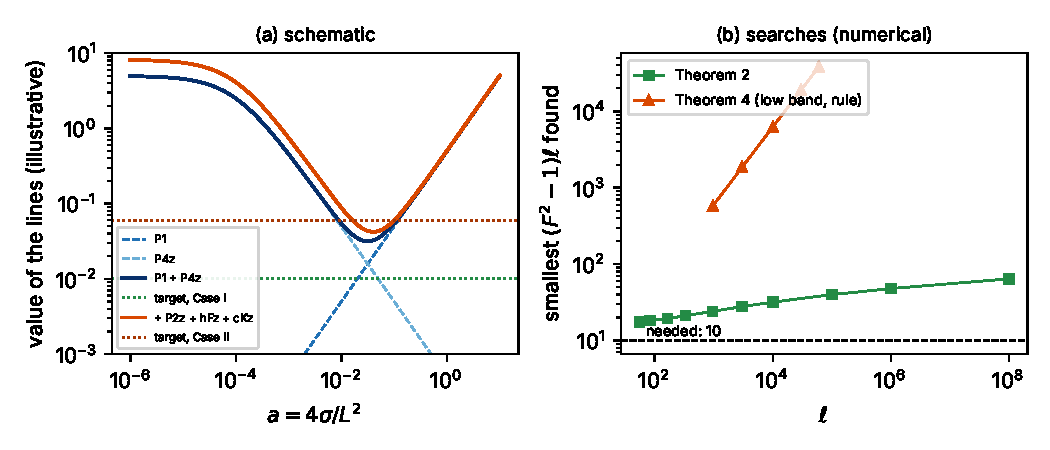
\includegraphics[width=\columnwidth]{figures/fig_cases.pdf}
\caption{(a) Schematic of the two cases of the rule, as functions of $a=4\sigma/L^2$ (log scale; illustrative values, not a state of the class). The background lines P1 and P4z have the sum $\ge\sqrt{b\omega}-\sigma/2$; in Case~I (dark ripple) it exceeds the target. In Case~II the ripple lines P2z, hFz and the chirp cKz are added. (b) The smallest $(F^2-1)\ell$ found by the searches of Sec.~\ref{sec:break}, where $F$ is the ratio of the best option to the target; the claim needs $10$. Squares: Theorem~\ref{thm:narrow}, all bands of $B$. Triangles: Theorem~\ref{thm:wide}, the band $8\ell+100\le B<5\times10^5$ (rule branch). \numst}
\label{fig:cases}
\end{figure}

\subsection{Where the hypotheses are used}

\begin{itemize}
\item No step uses a lower bound on $\mu$: small $\mu$ is handled by (m1)--(m2), where $\Theta^*$ grows like $1/\sqrt\mu$.
\item $B\ge2.5\times10^{10}$: in (R4), (b.2) and (b.5). $B\ge50(8\ell+100)$: to have $q\le0.0026$ and $z_2\le0.01$, i.e.\ coefficients of P2z and hFz close to one.
\item $a\le4r/\sigma$: in (R6)--(R7). $r\ge\sigma^3$: in (R1).
\item The boundary $\xi=\ell^2$ between (m3) and (m4) only splits the region; both are proofs of the same claim.
\end{itemize}

\subsection{The computer-assisted part}
\label{sec:ca}

The steps above are formulas.
That the $48$ quoted numbers and the $18$ conditions hold for \emph{every} $\ell\ge55.26$ is checked by interval arithmetic with outward rounding, on $[55.26,10^6]$ cut into $9{,}809$ geometric pieces of ratio $1.001$ and on the tail $[10^6,\infty)$ as one piece \caproofst{App.~\ref{app:C}}.
Functions that increase and decrease at once ($\ell^ke^{-\ell}$ and the like) are written through elementary functions whose monotonicity is proved by one derivative, so that the infinite tail gets a finite enclosure.
No piece fails.
The smallest margins are at $\ell=55.26$; for instance, Case~I with Fz has margin $0.004869$, Case~I with Tz-B2 $0.002545$, (II-ch) $0.004579$, and condition (N) $0.5845$; condition (N0) is tightest near $\ell=10^6$ with $4.93\times10^{-7}$.
The absorptions of (R1) and (R3) are a separate interval computation on $[55.26,\infty)$ as one piece: the sum of (R1) is at most $0.507288\,\mathrm{es}$ against $0.52\,\mathrm{es}$.
Table~\ref{tab:ca} lists every computer-assisted part of the paper.

The arithmetic uses Python's \code{decimal} with $40$ digits, widens every result outward by $10^{-38}$ relative, never uses the library power (which is not guaranteed to be correctly rounded in the C version), and refuses to invert an interval that contains $0$.
While the interval functions run, any rounding outside the interval context raises an exception (the \code{Inexact} flag of the default context is trapped); no exception occurs.
A test of $8{,}100$ random intervals and points against $90$-digit values finds no enclosure failure, and the same test catches each of four deliberately broken implementations.

\begin{table}
\caption{The computer-assisted parts of the paper. ``Pieces'' are intervals of $\ell$; the tail is $[10^6,\infty)$. All were run with the \code{Inexact} trap of the default context.}
\label{tab:ca}
\begin{ruledtabular}
\small
\begin{tabular}{p{0.34\columnwidth}p{0.27\columnwidth}p{0.24\columnwidth}}
what & how & code\\ \hline
48 numbers, 18 conditions of Proposition~\ref{prop:narrow} & 9,809 pieces $+$ tail & \code{dl\_consts.py}\\
absorptions (R1), (R3) & one piece $[55.26,\infty)$ & \code{dp\_r1.py}\\
constants and conditions of Proposition~\ref{prop:wide} & 6,952 pieces $+$ tail & \code{dp\_room1.py}, \code{dq\_room1\_low.py}\\
$M_4(10^{-4})\le2.0475$ (Lemma~\ref{lem:M4}) & pieces in $u$ & \code{dq\_m4.py}\\
$M_1(10^{-4})$, $M_2(10^{-4})$ (Lemma~\ref{lem:M12}) & pieces in $u$ & \code{du\_cl.py}\\
Theorem~H1 of~\cite{H} & certificates of~\cite{H} & repository of~\cite{H}\\
\end{tabular}
\end{ruledtabular}
\end{table}

\emph{Picture.}
With a narrow focus the observer sees a short piece of ripple.
If the ripple is dark, the background alone carries the information.
If it is bright, it cannot also hide at the centre of the focus; so it spreads, and its phase turns across the focus.
That turning, the chirp, is what pays.
The hardest states are where the ripple is just bright enough to need the chirp, and there the margin is $17.6/\ell$ at $\ell=55.26$, growing to $64/\ell$ at $\ell=10^8$ (Fig.~\ref{fig:cases}).
